\insertmeeting 
	{Github the G.O.A.T.} 
	{09/08/22}
	{Hagerty High School}
	{Anouska, Jensen, Jorge, Karissa, Laura, Mohana, Nathan, Ritam, Robert, Samantha, Tyler}
	{Images/RobotPics/robot.jpg}
	{2:30 - 4:00}
	
\hhscommittee{General}
\noindent\hfil\rule{\textwidth}{.4pt}\hfil
\subsubsection*{Goals}
\begin{itemize}
    \item Narrow down outreach possibilities
    \item Sign up and get connected with each other on Github and Onshape
\end{itemize} 

\noindent\hfil\rule{\textwidth}{.4pt}\hfil

\subsubsection*{Accomplishments}
In an earlier meeting, we organized various outreach ideas that we would be doing throughout the season. Since then, we've narrowed down which ideas we will actually be handling and today, we divided up the selected outreach ideas among the team members. This way, we have an idea of who would lead on the responsibility of contacting different industries and companies for outreach. Having a selected and labeled figurehead of each outreach task is more important than one would initially think. If it were out in the open to anyone who claims it, there is a chance multiple people might do the same task, but it's even more likely that it isn't done at all.

During the season, we will be using GItHub to share created code as well as to use code that was created in past FTC years. We use OnShape to create CAD models that are used on our robots. As such, it's important that we ensure all people have access to these very important resources. We updated our emails and usernames for Github and OnShape on a spreadsheet such that we can get everybody signed up and connected smoothly.



% \begin{figure}[htp]
% \centering
% 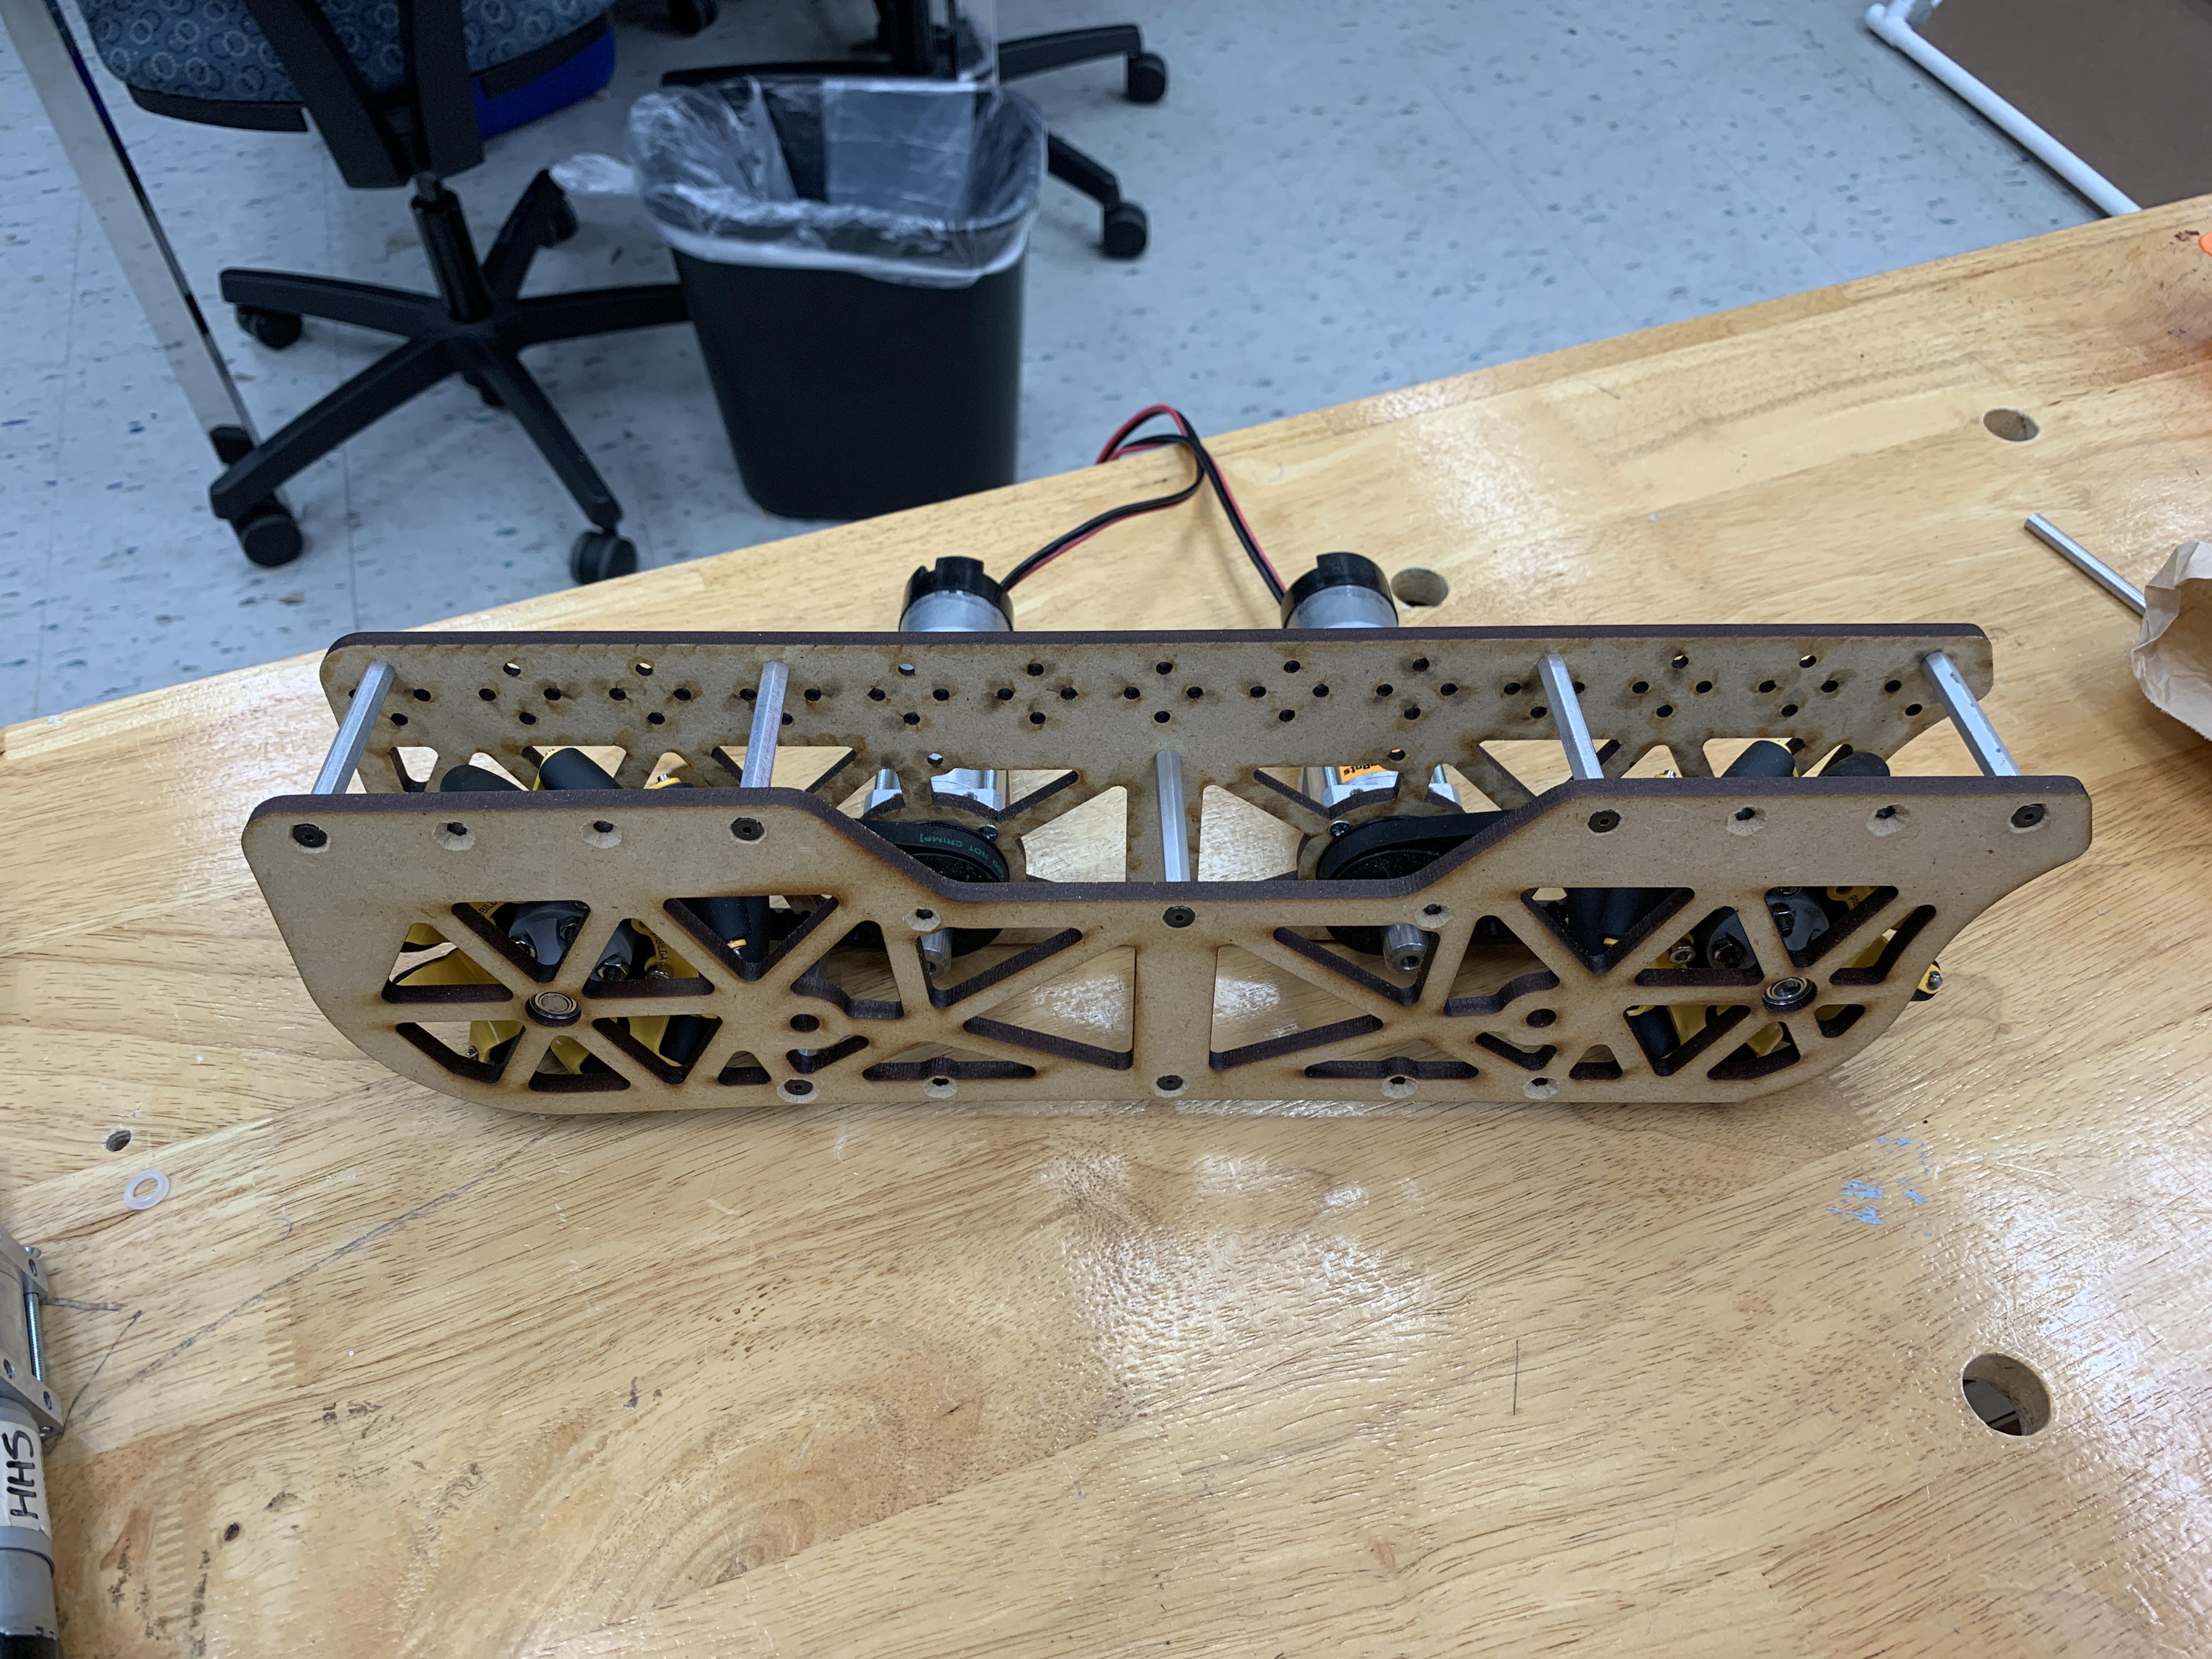
\includegraphics[width=0.9\textwidth, angle=0]{Meetings/July/07-21-21/drivetrain_7-20-21-NathanForrer.jpg}
% \caption{First half of the drivetrain.}
% \label{fig:072121_1}
% \end{figure}

\whatsnext{
\begin{itemize}
    \item Dicuss pre-season planning
	\item - Watch kickoff
\end{itemize} 
}
